% Options for packages loaded elsewhere
\PassOptionsToPackage{unicode}{hyperref}
\PassOptionsToPackage{hyphens}{url}
%
\documentclass[
]{article}
\usepackage{amsmath,amssymb}
\usepackage{lmodern}
\usepackage{ifxetex,ifluatex}
\ifnum 0\ifxetex 1\fi\ifluatex 1\fi=0 % if pdftex
  \usepackage[T1]{fontenc}
  \usepackage[utf8]{inputenc}
  \usepackage{textcomp} % provide euro and other symbols
\else % if luatex or xetex
  \usepackage{unicode-math}
  \defaultfontfeatures{Scale=MatchLowercase}
  \defaultfontfeatures[\rmfamily]{Ligatures=TeX,Scale=1}
\fi
% Use upquote if available, for straight quotes in verbatim environments
\IfFileExists{upquote.sty}{\usepackage{upquote}}{}
\IfFileExists{microtype.sty}{% use microtype if available
  \usepackage[]{microtype}
  \UseMicrotypeSet[protrusion]{basicmath} % disable protrusion for tt fonts
}{}
\makeatletter
\@ifundefined{KOMAClassName}{% if non-KOMA class
  \IfFileExists{parskip.sty}{%
    \usepackage{parskip}
  }{% else
    \setlength{\parindent}{0pt}
    \setlength{\parskip}{6pt plus 2pt minus 1pt}}
}{% if KOMA class
  \KOMAoptions{parskip=half}}
\makeatother
\usepackage{xcolor}
\IfFileExists{xurl.sty}{\usepackage{xurl}}{} % add URL line breaks if available
\IfFileExists{bookmark.sty}{\usepackage{bookmark}}{\usepackage{hyperref}}
\hypersetup{
  pdftitle={Final Project},
  pdfauthor={Zhengtao Xu, Jennings Cheng and Collin Carmichael},
  hidelinks,
  pdfcreator={LaTeX via pandoc}}
\urlstyle{same} % disable monospaced font for URLs
\usepackage[margin=1in]{geometry}
\usepackage{color}
\usepackage{fancyvrb}
\newcommand{\VerbBar}{|}
\newcommand{\VERB}{\Verb[commandchars=\\\{\}]}
\DefineVerbatimEnvironment{Highlighting}{Verbatim}{commandchars=\\\{\}}
% Add ',fontsize=\small' for more characters per line
\usepackage{framed}
\definecolor{shadecolor}{RGB}{248,248,248}
\newenvironment{Shaded}{\begin{snugshade}}{\end{snugshade}}
\newcommand{\AlertTok}[1]{\textcolor[rgb]{0.94,0.16,0.16}{#1}}
\newcommand{\AnnotationTok}[1]{\textcolor[rgb]{0.56,0.35,0.01}{\textbf{\textit{#1}}}}
\newcommand{\AttributeTok}[1]{\textcolor[rgb]{0.77,0.63,0.00}{#1}}
\newcommand{\BaseNTok}[1]{\textcolor[rgb]{0.00,0.00,0.81}{#1}}
\newcommand{\BuiltInTok}[1]{#1}
\newcommand{\CharTok}[1]{\textcolor[rgb]{0.31,0.60,0.02}{#1}}
\newcommand{\CommentTok}[1]{\textcolor[rgb]{0.56,0.35,0.01}{\textit{#1}}}
\newcommand{\CommentVarTok}[1]{\textcolor[rgb]{0.56,0.35,0.01}{\textbf{\textit{#1}}}}
\newcommand{\ConstantTok}[1]{\textcolor[rgb]{0.00,0.00,0.00}{#1}}
\newcommand{\ControlFlowTok}[1]{\textcolor[rgb]{0.13,0.29,0.53}{\textbf{#1}}}
\newcommand{\DataTypeTok}[1]{\textcolor[rgb]{0.13,0.29,0.53}{#1}}
\newcommand{\DecValTok}[1]{\textcolor[rgb]{0.00,0.00,0.81}{#1}}
\newcommand{\DocumentationTok}[1]{\textcolor[rgb]{0.56,0.35,0.01}{\textbf{\textit{#1}}}}
\newcommand{\ErrorTok}[1]{\textcolor[rgb]{0.64,0.00,0.00}{\textbf{#1}}}
\newcommand{\ExtensionTok}[1]{#1}
\newcommand{\FloatTok}[1]{\textcolor[rgb]{0.00,0.00,0.81}{#1}}
\newcommand{\FunctionTok}[1]{\textcolor[rgb]{0.00,0.00,0.00}{#1}}
\newcommand{\ImportTok}[1]{#1}
\newcommand{\InformationTok}[1]{\textcolor[rgb]{0.56,0.35,0.01}{\textbf{\textit{#1}}}}
\newcommand{\KeywordTok}[1]{\textcolor[rgb]{0.13,0.29,0.53}{\textbf{#1}}}
\newcommand{\NormalTok}[1]{#1}
\newcommand{\OperatorTok}[1]{\textcolor[rgb]{0.81,0.36,0.00}{\textbf{#1}}}
\newcommand{\OtherTok}[1]{\textcolor[rgb]{0.56,0.35,0.01}{#1}}
\newcommand{\PreprocessorTok}[1]{\textcolor[rgb]{0.56,0.35,0.01}{\textit{#1}}}
\newcommand{\RegionMarkerTok}[1]{#1}
\newcommand{\SpecialCharTok}[1]{\textcolor[rgb]{0.00,0.00,0.00}{#1}}
\newcommand{\SpecialStringTok}[1]{\textcolor[rgb]{0.31,0.60,0.02}{#1}}
\newcommand{\StringTok}[1]{\textcolor[rgb]{0.31,0.60,0.02}{#1}}
\newcommand{\VariableTok}[1]{\textcolor[rgb]{0.00,0.00,0.00}{#1}}
\newcommand{\VerbatimStringTok}[1]{\textcolor[rgb]{0.31,0.60,0.02}{#1}}
\newcommand{\WarningTok}[1]{\textcolor[rgb]{0.56,0.35,0.01}{\textbf{\textit{#1}}}}
\usepackage{graphicx}
\makeatletter
\def\maxwidth{\ifdim\Gin@nat@width>\linewidth\linewidth\else\Gin@nat@width\fi}
\def\maxheight{\ifdim\Gin@nat@height>\textheight\textheight\else\Gin@nat@height\fi}
\makeatother
% Scale images if necessary, so that they will not overflow the page
% margins by default, and it is still possible to overwrite the defaults
% using explicit options in \includegraphics[width, height, ...]{}
\setkeys{Gin}{width=\maxwidth,height=\maxheight,keepaspectratio}
% Set default figure placement to htbp
\makeatletter
\def\fps@figure{htbp}
\makeatother
\setlength{\emergencystretch}{3em} % prevent overfull lines
\providecommand{\tightlist}{%
  \setlength{\itemsep}{0pt}\setlength{\parskip}{0pt}}
\setcounter{secnumdepth}{-\maxdimen} % remove section numbering
\ifluatex
  \usepackage{selnolig}  % disable illegal ligatures
\fi

\title{Final Project}
\author{Zhengtao Xu, Jennings Cheng and Collin Carmichael}
\date{7/22/2021}

\begin{document}
\maketitle

\textbf{Introduction}

\textbf{Exploratory Data Analysis}

\begin{verbatim}
##                Avg_Day_PM2.5 Avg_Day_DEWP Avg_Day_TEMP Avg_Day_PRES
## Avg_Day_PM2.5     1.00000000   0.14859422  -0.08398145  -0.02806745
## Avg_Day_DEWP      0.14859422   1.00000000   0.90522215  -0.80034407
## Avg_Day_TEMP     -0.08398145   0.90522215   1.00000000  -0.86484298
## Avg_Day_PRES     -0.02806745  -0.80034407  -0.86484298   1.00000000
## Max_Day_LWS      -0.33435302  -0.38341283  -0.23591663   0.21860730
## Avg_Day_PRES.1   -0.02806745  -0.80034407  -0.86484298   1.00000000
## Max_Day_LWS.1    -0.33435302  -0.38341283  -0.23591663   0.21860730
## Max_Day_LS        0.06214689  -0.08024689  -0.18682393   0.14597490
## Max_Day_LR       -0.03932810   0.29779563   0.18845351  -0.20593980
##                 Max_Day_LWS Avg_Day_PRES.1 Max_Day_LWS.1   Max_Day_LS
## Avg_Day_PM2.5  -0.334353016    -0.02806745  -0.334353016  0.062146893
## Avg_Day_DEWP   -0.383412827    -0.80034407  -0.383412827 -0.080246894
## Avg_Day_TEMP   -0.235916629    -0.86484298  -0.235916629 -0.186823931
## Avg_Day_PRES    0.218607303     1.00000000   0.218607303  0.145974900
## Max_Day_LWS     1.000000000     0.21860730   1.000000000 -0.009822741
## Avg_Day_PRES.1  0.218607303     1.00000000   0.218607303  0.145974900
## Max_Day_LWS.1   1.000000000     0.21860730   1.000000000 -0.009822741
## Max_Day_LS     -0.009822741     0.14597490  -0.009822741  1.000000000
## Max_Day_LR     -0.062115316    -0.20593980  -0.062115316 -0.025754440
##                 Max_Day_LR
## Avg_Day_PM2.5  -0.03932810
## Avg_Day_DEWP    0.29779563
## Avg_Day_TEMP    0.18845351
## Avg_Day_PRES   -0.20593980
## Max_Day_LWS    -0.06211532
## Avg_Day_PRES.1 -0.20593980
## Max_Day_LWS.1  -0.06211532
## Max_Day_LS     -0.02575444
## Max_Day_LR      1.00000000
\end{verbatim}

\begin{verbatim}
## 
## Call:
## lm(formula = Avg_Day_PM2.5 ~ ., data = Pollution_Daily.train)
## 
## Residuals:
##     Min      1Q  Median      3Q     Max 
## -159.14  -40.87  -10.04   29.32  321.50 
## 
## Coefficients:
##                  Estimate Std. Error t value Pr(>|t|)    
## (Intercept)    -4.615e+06  2.113e+06  -2.184 0.029089 *  
## Date_D         -6.411e+00  2.935e+00  -2.184 0.029129 *  
## Avg_Day_DEWP    7.189e+00  3.627e-01  19.821  < 2e-16 ***
## Avg_Day_TEMP   -1.081e+01  4.737e-01 -22.824  < 2e-16 ***
## Avg_Day_PRES   -2.504e+00  3.322e-01  -7.539 8.43e-14 ***
## Max_Day_LWS    -1.646e-01  2.730e-02  -6.030 2.08e-09 ***
## Max_Day_LS     -4.196e+00  1.016e+00  -4.132 3.81e-05 ***
## Max_Day_LR     -5.354e+00  6.344e-01  -8.440  < 2e-16 ***
## Max_Day_CBWDNE -7.925e+01  1.803e+01  -4.395 1.19e-05 ***
## Max_Day_CBWDNW -5.632e+01  1.677e+01  -3.359 0.000803 ***
## Max_Day_CBWDSE -5.075e+01  1.670e+01  -3.038 0.002424 ** 
## Year            2.344e+03  1.072e+03   2.186 0.028992 *  
## Month           1.933e+02  8.935e+01   2.163 0.030699 *  
## Day             7.128e+00  2.934e+00   2.430 0.015231 *  
## ---
## Signif. codes:  0 '***' 0.001 '**' 0.01 '*' 0.05 '.' 0.1 ' ' 1
## 
## Residual standard error: 61.18 on 1420 degrees of freedom
##   (26 observations deleted due to missingness)
## Multiple R-squared:  0.4062, Adjusted R-squared:  0.4007 
## F-statistic: 74.71 on 13 and 1420 DF,  p-value: < 2.2e-16
\end{verbatim}

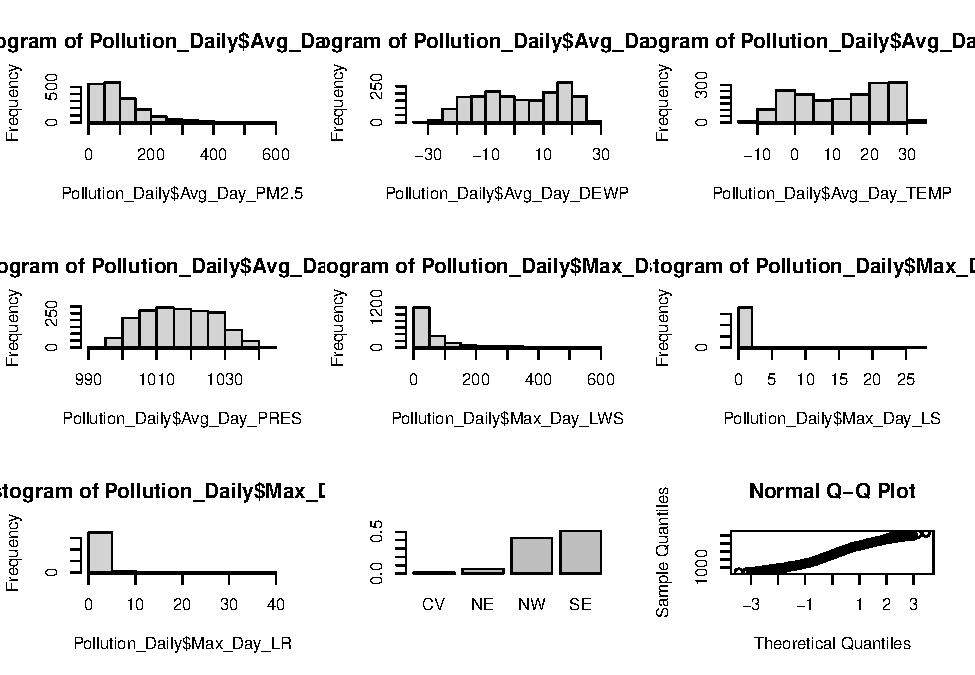
\includegraphics{Final_Project_1_files/figure-latex/unnamed-chunk-4-1.pdf}

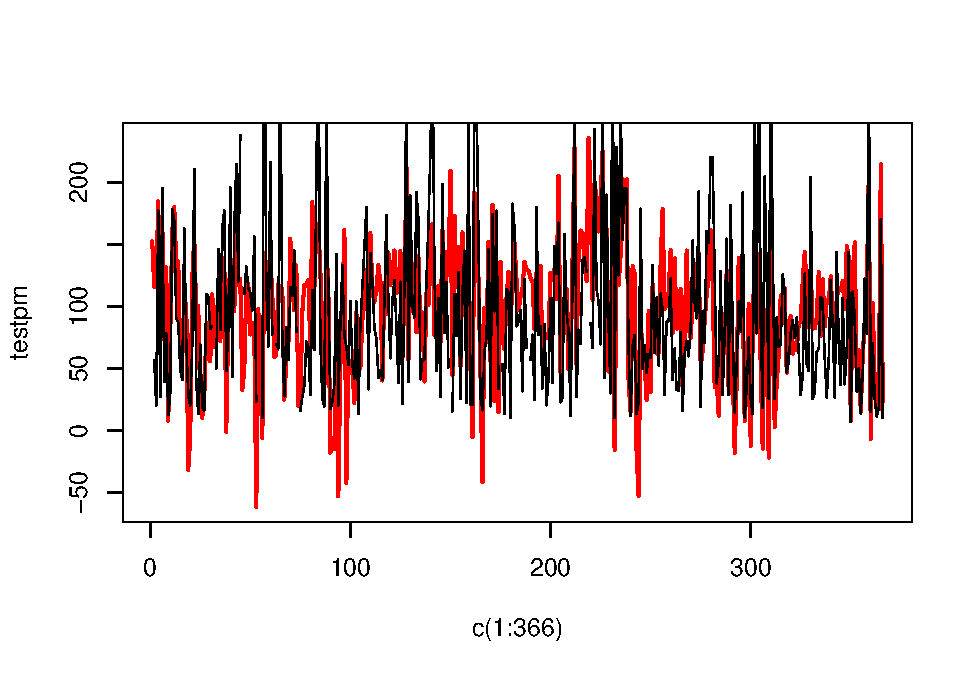
\includegraphics{Final_Project_1_files/figure-latex/unnamed-chunk-6-1.pdf}

\begin{Shaded}
\begin{Highlighting}[]
\FunctionTok{test\_error\_assumptions}\NormalTok{(lm\_all)}
\end{Highlighting}
\end{Shaded}

\begin{verbatim}
##    X.Homocedasticity. b...0.05 X.Normality. c...0.05 X.Uncorrelated.Errors.
## BP    Homocedasticity    FALSE    Normality    FALSE    Uncorrelated Errors
##    d...0.05
## BP    FALSE
\end{verbatim}

\begin{Shaded}
\begin{Highlighting}[]
\FunctionTok{test\_influence}\NormalTok{(lm\_all)}
\end{Highlighting}
\end{Shaded}

\begin{verbatim}
## [1] b
## <0 rows> (or 0-length row.names)
\end{verbatim}

\begin{Shaded}
\begin{Highlighting}[]
\FunctionTok{test\_leverage}\NormalTok{(lm\_all)}
\end{Highlighting}
\end{Shaded}

\begin{verbatim}
##          3          9         35         38         42         43         45 
## 0.18312369 0.01993036 0.02084889 0.02909985 0.02120462 0.02016636 0.01957692 
##         59         60         65         67         73        112        118 
## 0.02778616 0.02873632 0.02280094 0.04509421 0.05684717 0.02384532 0.02513578 
##        119        148        212        250        260        264        297 
## 0.02561832 0.04775556 0.02202594 0.01983728 0.07229409 0.02603939 0.03053323 
##        347        355        364        365        372        375        404 
## 0.02136388 0.08376838 0.02120852 0.04800714 0.03052893 0.02213194 0.02044289 
##        409        417        423        465        470        575        608 
## 0.04888755 0.07645773 0.02899026 0.02330743 0.01974735 0.02305260 0.02132032 
##        618        659        664        702        717        725        734 
## 0.03280053 0.07335589 0.07415222 0.02154804 0.01978184 0.02197048 0.02104081 
##        737        758        760        792        808        894        918 
## 0.08265230 0.07757221 0.02815190 0.04180265 0.02611715 0.02164709 0.02029063 
##        933        934        939        943        944       1017       1018 
## 0.02844410 0.04995945 0.01991536 0.03709670 0.04839376 0.07291344 0.07278236 
##       1019       1039       1040       1044       1064       1065       1077 
## 0.07320367 0.10636050 0.03250507 0.07316761 0.01984485 0.01984594 0.02111622 
##       1079       1098       1099       1119       1125       1128       1129 
## 0.09675365 0.02018495 0.02925196 0.02134172 0.02862577 0.02008693 0.01977021 
##       1130       1175       1183       1292       1362       1370       1375 
## 0.03647560 0.02881126 0.02004238 0.05664320 0.02051762 0.02092169 0.07448111 
##       1428       1429       1434       1449       1454       1457       1463 
## 0.03298086 0.03492779 0.01996232 0.01966219 0.07518163 0.02553009 0.07930188 
##       1485       1499       1500       1555       1592       1654       1677 
## 0.02054096 0.08190632 0.13694349 0.02033825 0.03754080 0.01992540 0.02158615 
##       1703       1727       1743       1772       1792       1797 
## 0.02238124 0.05105359 0.07468200 0.07520319 0.01981613 0.02760467
\end{verbatim}

\begin{Shaded}
\begin{Highlighting}[]
\FunctionTok{test\_outlier}\NormalTok{(lm\_all)}
\end{Highlighting}
\end{Shaded}

\begin{verbatim}
##             b d        c
## 417  4.416884 > 4.152357
## 1108 5.333325 > 4.152357
## 1477 4.792634 > 4.152357
## 1517 4.647787 > 4.152357
## 1518 4.233889 > 4.152357
\end{verbatim}

\begin{Shaded}
\begin{Highlighting}[]
\DocumentationTok{\#\#Checking Interaction Term Significance}
\FunctionTok{anova}\NormalTok{(lm\_all)}
\end{Highlighting}
\end{Shaded}

\begin{verbatim}
## Analysis of Variance Table
## 
## Response: Avg_Day_PM2.5
##                Df  Sum Sq Mean Sq  F value    Pr(>F)    
## Date_D          1    1339    1339   0.3577 0.5499001    
## Avg_Day_DEWP    1  188302  188302  50.3013 2.073e-12 ***
## Avg_Day_TEMP    1 2395516 2395516 639.9164 < 2.2e-16 ***
## Avg_Day_PRES    1  244962  244962  65.4370 1.275e-15 ***
## Max_Day_LWS     1  232063  232063  61.9912 6.801e-15 ***
## Max_Day_LS      1   38629   38629  10.3189 0.0013463 ** 
## Max_Day_LR      1  293980  293980  78.5312 < 2.2e-16 ***
## Max_Day_CBWD    3  110235   36745   9.8158 2.076e-06 ***
## Year            1   44499   44499  11.8871 0.0005818 ***
## Month           1   64290   64290  17.1739 3.612e-05 ***
## Day             1   22101   22101   5.9038 0.0152314 *  
## Residuals    1420 5315745    3743                       
## ---
## Signif. codes:  0 '***' 0.001 '**' 0.01 '*' 0.05 '.' 0.1 ' ' 1
\end{verbatim}

\end{document}
